\documentclass[10pt,tikz,border=1mm]{standalone} 
\usepackage{mathpazo}
\usepackage[T1]{fontenc}
\usetikzlibrary{calc}
\tikzstyle{process}=[rectangle,minimum height=1.5cm,minimum width=2.5cm,fill=black!5,draw=black, thick]
\tikzstyle{arrow}=[->,>=stealth,thin,text=black,font=\normalsize]
\begin{document}
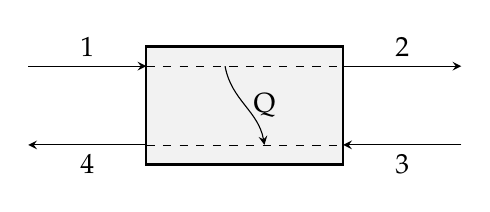
\begin{tikzpicture}
	%\draw[step=0.5cm,black!20,very thin] (0,0) grid (6,2);
	\node [process] at (2.75,0.75) {};
	\coordinate (A) at (0,1.25);
	\coordinate (B) at (0,0.25);
	\coordinate (A1) at (1.5,1.25);
	\coordinate (B1) at (1.5,0.25);
	\coordinate (C) at (4,1.25);
	\coordinate (D) at (4,0.25);
	\coordinate (C1) at (5.5,1.25);
	\coordinate (D1) at (5.5,0.25);
	\coordinate (Q1) at (2.5,1.25);
	\coordinate (Q2) at (3,0.25);
	\draw[arrow] (A) -- node[above]{1} (A1);
	\draw[arrow] (B1) -- node[below]{4} (B);
	\draw[arrow] (C) -- node[above]{2} (C1);
	\draw[arrow] (D1) -- node[below]{3} (D);
	\draw[dashed,very thin] (A1) -- (C);
	\draw[dashed,very thin] (B1) -- (D);
	\draw[arrow] (Q1) to [out=280,in=100] (Q2);
	\node at (3,0.75) {Q};
\end{tikzpicture}
\end{document}